% The document class supplies options to control rendering of some standard
% features in the result.  The goal is for uniform style, so some attention 
% to detail is *vital* with all fields.  Each field (i.e., text inside the
% curly braces below, so the MEng text inside {MEng} for instance) should 
% take into account the following:
%
% - author name       should be formatted as "FirstName LastName"
%   (not "Initial LastName" for example),
% - supervisor name   should be formatted as "Title FirstName LastName"
%   (where Title is "Dr." or "Prof." for example),
% - degree programme  should be "BSc", "MEng", "MSci", "MSc" or "PhD",
% - dissertation title should be correctly capitalised (plus you can have
%   an optional sub-title if appropriate, or leave this field blank),
% - dissertation type should be formatted as one of the following:
%   * for the MEng degree programme either "enterprise" or "research" to
%     reflect the stream,
%   * for the MSc  degree programme "$X/Y/Z$" for a project deemed to be
%     X%, Y% and Z% of type I, II and III.
% - year              should be formatted as a 4-digit year of submission
%   (so 2014 rather than the academic year, say 2013/14 say).

\documentclass[ oneside,% the name of the author
                    author={Joshua Felmeden},
                % the degree programme: BSc, MEng, MSci or MSc.
                    degree={MEng},
                % the dissertation    title (which cannot be blank)
                     title={Semantic Analysis of Financial Headlines Based on Realised Stock Returns},
                % the dissertation subtitle (which can    be blank)
                  subtitle={}]{dissertation}

\usepackage{booktabs}
\usepackage{multirow}
\usepackage{subcaption}
\begin{document}

% =============================================================================

% This section simply introduces the structural guidelines.  It can clearly
% be deleted (or commented out) if you use the file as a template for your
% own dissertation: everything following it is in the correct order to use 
% as is.

\section*{Prelude}
\thispagestyle{empty}

A typical dissertation will be structured according to (somewhat) standard 
sections, described in what follows.  However, it is hard and perhaps even 
counter-productive to generalise: the goal is {\em not} to be prescriptive, 
but simply to act as a guideline.  In particular, each page count given is
important but {\em not} absolute: their aim is simply to highlight that a 
clear, concise description is better than a rambling alternative that makes
it hard to separate important content and facts from trivia.

% You can use this document as a \LaTeX-based~\cite{latexbook1,latexbook2} 
template for your own dissertation by simply deleting extraneous sections
and content; keep in mind that the associated {\tt Makefile} could be of
use. %, in particular because it automatically executes \mbox{\BibTeX} to 
deal with the associated bibliography. 
Alternatively, upload this template, dissertation.bib, dissertation.cls, 
dtklogos.sty and the "logo" folder to Overleaf (an online \LaTeX editor and compiler) and work on your thesis there.

\textbf{Do not include this section in your final dissertation --- just delete it from the source.}

% =============================================================================

% This macro creates the standard UoB title page by using information drawn
% from the document class (meaning it is vital you select the correct degree 
% title and so on).

\maketitle

% After the title page (which is a special case in that it is not numbered)
% comes the front matter or preliminaries; this macro signals the start of
% such content, meaning the pages are numbered with Roman numerals.

\frontmatter


%\lstlistoflistings

% The following sections are part of the front matter, but are not generated
% automatically by LaTeX; the use of \chapter* means they are not numbered.

% -----------------------------------------------------------------------------

\chapter*{Abstract}

{\bf A compulsory section, of at most 300 words} 
\vspace{1cm} 

\noindent
This section should pr\'{e}cis the project context, aims and objectives,
and main contributions (e.g., deliverables) and achievements; the same 
section may be called an abstract elsewhere.  The goal is to ensure the 
reader is clear about what the topic is, what you have done within this 
topic, {\em and} what your view of the outcome is.

The former aspects should be guided by your specification: essentially 
this section is a (very) short version of what is typically the first 
chapter. If your project is experimental in nature, this should include 
a clear research hypothesis.  This will obviously differ significantly
for each project, but an example might be as follows:

\begin{quote}
My research hypothesis is that a suitable genetic algorithm will yield
more accurate results (when applied to the standard ACME data set) than 
the algorithm proposed by Jones and Smith, while also executing in less
time.
\end{quote}

\noindent
The latter aspects should (ideally) be presented as a concise, factual 
bullet point list.  Again the points will differ for each project, but 
an might be as follows:

\begin{quote}
\noindent
\begin{itemize}
\item I spent $120$ hours collecting material on and learning about the 
      Java garbage-collection sub-system. 
\item I wrote a total of $5000$ lines of source code, comprising a Linux 
      device driver for a robot (in C) and a GUI (in Java) that is 
      used to control it.
\item I designed a new algorithm for computing the non-linear mapping 
      from A-space to B-space using a genetic algorithm, see page $17$.
\item I implemented a version of the algorithm proposed by Jones and 
      Smith in [6], see page $12$, corrected a mistake in it, and 
      compared the results with several alternatives.
\end{itemize}
\end{quote}

% -----------------------------------------------------------------------------


\chapter*{Dedication and Acknowledgements}

{\bf A compulsory section}
\vspace{1cm} 

\noindent
It is common practice (although totally optional) to acknowledge any
third-party advice, contribution or influence you have found useful
during your work.  Examples include support from friends or family, 
the input of your Supervisor and/or Advisor, external organisations 
or persons who  have supplied resources of some kind (e.g., funding, 
advice or time), and so on.


% -----------------------------------------------------------------------------


\chapter*{COVID-19 Statement}

{\bf An optional section, of at most 800 words} 
\vspace{1cm} 

\noindent
A summary of any planned research activities disrupted by Covid-19 restrictions and the extent to which it was possible to adapt the work in those changed circumstances. If the project was able to go forward as planned, you can safely remove this section without losing any marks. The following may be included:

\begin{itemize}
\item Details of any planned research activities curtailed by the pandemic because of, for example, lack of access to facilities, libraries, archives, research participants, fieldwork, etc. Information on any curtailed training should be included only insofar as it relates to the impact on research activities and on the dissertation.

\item An acknowledgement of the anticipated contribution and value to the dissertation if those research activities had not been curtailed and what was possible to include in the dissertation in the circumstances, including where alternative choices were made to adapt the work and whether there are any weaknesses that could not be overcome.

\item Any other relevant factors on the impact of Covid-19 on research activities and on the contents of the dissertation.

\item Details of any research activities required by the examiners as part of a resubmission that were curtailed by the pandemic may be included in a new or revised Covid-19 statement in the resubmitted dissertation.
\end{itemize}

% -----------------------------------------------------------------------------

% This macro creates the standard UoB declaration; on the printed hard-copy,
% this must be physically signed by the author in the space indicated.

\makedecl



% -----------------------------------------------------------------------------

% LaTeX automatically generates a table of contents, plus associated lists 
% of figures and tables.  These are all compulsory parts of the dissertation.

\tableofcontents
\listoffigures
\listoftables

% -----------------------------------------------------------------------------



\chapter*{Ethics Statement}

{\bf A compulsory section} 
\vspace{1cm} 

In almost every project, this will be one of the following statements:
    \begin{itemize}
        \item ``This project did not require ethical review, as determined by my supervisor, [fill in name]''; or
        \item ``This project fits within the scope of ethics application 0026, as reviewed by my supervisor, [fill in name]''; or
        \item ``An ethics application for this project was reviewed and approved by the faculty research ethics committee as application [fill in number]''.
    \end{itemize}
    
See Section 3.2 of the unit Handbook for more information. If something went wrong and none of those three statements apply, then you should instead explain what happened.


% -----------------------------------------------------------------------------

\chapter*{Summary of Changes}

{\bf A conditional section} 
\vspace{1cm} 

If and only if the dissertation represents a resubmission (e.g., as the result of
a resit), this section is compulsory: the content should summarise all
non-trivial changes made to the initial submission.  Otherwise you can
omit it, since a summary of this type is clearly nonsensical.

When included, the section will ideally be used to highlight additional
work completed, and address criticism raised in any associated feedback.
Clearly it is difficult to give generic advice about how to do so, but
an example might be as follows:

\begin{quote}
\noindent
\begin{itemize}
\item Feedback from the initial submission criticised the design and 
      implementation of my genetic algorithm, stating ``there seems 
      to have been no attention to computational complexity during the
      design, and obvious methods of optimisation are missing within
      the resulting implementation''.  Chapter $3$ now includes a
      comprehensive analysis of the algorithm, in terms of both time
      and space.  While I have not altered the algorithm itself, I
      have included a cache mechanism (also detailed in Chapter $3$)
      that provides a significant improvement in average run-time.
\item I added a feature in my implementation to allow automatic rather
      than manual selection of various parameters; the experimental
      results in Chapter $4$ have been updated to reflect this.
\item Questions after the presentation highlighted a range of related
      work that I had not considered: I have make a number of updates 
      to Chapter $2$, resolving this issue.
\end{itemize}
\end{quote}

% -----------------------------------------------------------------------------

\chapter*{Supporting Technologies}

{\bf An optional section}
\vspace{1cm} 

\noindent
This section should present a detailed summary, in bullet point form, 
of any third-party resources (e.g., hardware and software components) 
used during the project.  Use of such resources is always perfectly 
acceptable: the goal of this section is simply to be clear about how
and where they are used, so that a clear assessment of your work can
result.  The content can focus on the project topic itself (rather,
for example, than including ``I used \mbox{\LaTeX} to prepare my 
dissertation''); an example is as follows:

\begin{quote}
\noindent
\begin{itemize}
\item I used the Java {\tt BigInteger} class to support my implementation 
      of RSA.
\item I used a parts of the OpenCV computer vision library to capture 
      images from a camera, and for various standard operations (e.g., 
      threshold, edge detection).
\item I used an FPGA device supplied by the Department, and altered it 
      to support an open-source UART core obtained from 
      \url{http://opencores.org/}.
\item The web-interface component of my system was implemented by 
      extending the open-source WordPress software available from
      \url{http://wordpress.org/}.
\end{itemize}
\end{quote}

% -----------------------------------------------------------------------------

\chapter*{Notation and Acronyms}

\begin{quote}
\noindent
\begin{tabular}{lcl}
NLP               &:    &     Natural Language Processing \\
SESTM             &:    &     Semantic Extraction via Screening and Topic Modelling \\
\\
\textbf{SESTM Specific Notation} \\
$m$               &:    &     Number of words in sample \\
$n$               &:    &     Number of articles in sample \\
$d_{i,j}$         &:    &     Number of times word $j$ appears in text $i$ \\
$d_{[S],i}$       &:    &     Subset of columns where the only indices are those with sentiment \\
$D = [d_1, \dots, d_n]$ &:    & $m \times n$ Document term matrix \\
$sgn(y)$          &:    &     Sign of returns of article y \\
$\hat x$          &:    &    Expected value of variable $x$ \\
\end{tabular}
\end{quote}


% =============================================================================

% After the front matter comes a number of chapters; under each chapter,
% sections, subsections and even subsubsections are permissible.  The
% pages in this part are numbered with Arabic numerals.  Note that:
%
% - A reference point can be marked using \label{XXX}, and then later
%   referred to via \ref{XXX}; for example Chapter\ref{chap:context}.
% - The chapters are presented here in one file; this can become hard
%   to manage.  An alternative is to save the content in seprate files
%   the use \input{XXX} to import it, which acts like the #include
%   directive in C.

\mainmatter


\chapter{Introduction}
\label{chap:context}
Financial news is a widely available resource from which many investors, businesses and <idk> glean information. It is an insight into how many different businesses function and the health of markets and, if properly used, can be taken as a measure of ... Analysing the sentiment of an article has been used for a significant amount of time and is utilised for a myriad of purposes, including forecasting financial stocks.

An article is naturally formed of two parts, the headline and the article body. The bulk of the information conveyed by a given article is in the body, however, since headlines are often a summarisation of the body, it has been proven that data mining from the headline itself can be at least as useful as mining the body \{citation needed\}. The average word counts of a headline are very low, however, the vocabulary is often much higher impact on average, as this is what initially grabs the attention of a reader.

\section{What to do}

\noindent
This chapter should introduce the project context and motivate each of the proposed aims and objectives.  Ideally, it is written at a fairly high-level, and easily understood by a reader who is technically competent but not an expert in the topic itself.

In short, the goal is to answer three questions for the reader.  First, what is the project topic, or problem being investigated?  Second, why is the topic important, or rather why should the reader care about it?  For example, why there is a need for this project (e.g., lack of similar software or deficiency in existing software), who will benefit from the project and in what way (e.g., end-users, or software developers) what work does the project build on and why is the selected approach either important and/or interesting (e.g., fills a gap in literature, applies results from another field to a new problem).  Finally, what are the central challenges involved and why are they significant? 
 
The chapter should conclude with a concise bullet point list that summarises the aims and objectives.  For example:

\begin{quote}
\noindent
The high-level objective of this project is to reduce the performance 
gap between hardware and software implementations of modular arithmetic.  
More specifically, the concrete aims are:

\begin{enumerate}
\item Research and survey literature on public-key cryptography and
      identify the state of the art in exponentiation algorithms.
\item Improve the state of the art algorithm so that it can be used
      in an effective and flexible way on constrained devices.
\item Implement a framework for describing exponentiation algorithms
      and populate it with suitable examples from the literature on 
      an ARM7 platform.
\item Use the framework to perform a study of algorithm performance
      in terms of time and space, and show the proposed improvements
      are worthwhile.
\end{enumerate}
\end{quote}

% -----------------------------------------------------------------------------

\chapter{Background}
\label{chap:technical}

We begin by discussing the technical background that relate to the work in the thesis. This project evaluates and analyses the success of semantic analysis when applied to financial headlines; making use of realised stock returns as a teaching signal.

\section{Semantic Analysis}
Semantic analysis (also known as opinion mining) is the task of identifying opinions or sentiment of authors from an input of text. The ramifications of being able to programmatically extract the intended meaning of an input is extremely powerful in a variety of fields and is particularly prudent in a financial context. The nuances of natural language can sometimes make this difficult to extract, and therefore significant research has been conducted on the topic over the course of the last decades. The main fields of sentiment analysis are lexicon based, and deep learning based.


\subsection{Lexicon Based Methods}
The fundamental concept revolves around investigating a piece of text, and deciding on a binary classification: positive or negative. The simplest method compiles a list words with weights. Each weight corresponds to the positivity of the word (for example `great' would have a high positivity, while `terrible' would have very low). The overall sentiment of a piece of text could then be estimated by summing the individual sentiment scores of each word. The dictionary is not limited to single words, and can be expanded to include $n$-grams (phrases of $n$ words), as the context in which a word is used can dramatically change the sentiment. This may increase the accuracy of the dictionary at the cost of increased dimensionality. The dictionary itself must be compiled before it is possible to utilise this method. One of the most widely used for English text is the Harvard-IV-4 TagNeg (H4N) lexicon which is a general usage model that can be used to estimate the sentiment of a piece of text.

There are many difficulties faced with creating a dictionary of this sort, as language is often a subjective entity, leading to conflicting opinions in assigning tone to a specific word. Furthermore, the context within which a word is used can drastically change the intended sentiment of a word, for example, the word `great' is naturally a very positive word, however, if used in a sarcastic manner (e.g. `It's so great that my flight is delayed!') can invert the sentiment entirely. For this reason, simply summing the sentiment of a piece of text on a word by word scale can give an incorrect estimate.

Certain words that may have no meaning at all in one context, may have significant sentiment in another, particularly in the field of finance, where jargon dominates text. Loughran and McDonald \cite{lm-dict} conducted an investigation into the use of standard lexicons for use in analysing 10-K filing reports, which are comprehensive reports filed by companies about their financial performance. They discovered that almost 75\% of negative words found in the filings based on the H4N file were not typically negative in a financial context. For example, `liability' is a negatively charged word in a standard context, while it carries no tone at all in the context of the filings. Loughran and McDonald created their own dictionary based on these results called the Loughran McDonald dictionary that is created for the purpose of classifying 10-k filings. For these reasons, lexicon based methods work far better if the it is bespoke for the topic at hand, needing a specific dictionary for each task. 

\subsection{Deep Learning Methods}
Deep learning is at the forefront of innovation within the field of computer science and is being applied to increasingly complex problems that were once thought impossible for machines to complete. Naturally, its application in sentiment analysis and NLP has also been explored to some success in recent years.

Discussing the intricacies of modern deep learning methods is out of the scope of this paper, but an overview is sufficient to understand the motives behind the techniques used. Simply, deep learning uses multiple layers of non-linear processing units for feature extraction. Lower layers learn simple features, while those higher up build on this understanding and learn more complex features. In NLP terms, the models need \textit{word embedding} results as input features 

\section{Semantic Extraction via Screening and Topic Modelling}
Semantic Extraction via Screening and topic model (SESTM) is a novel text mining algorithm that makes us of a teaching signal developed by Zhang et Al. in 2020. It makes use of stock returns as a teaching signal to develop a model of sentiment words in maximally positive or negative arguments in order to be able to predict the sentiment of out of sample articles.

\subsection{Generating the sample}
\begin{itemize}
      \item Discuss aligning hte article with returns
      \begin{itemize}
            \item Discuss private stocks and public stocks
            \item Discuss non market days
      \end{itemize}
      \item Discuss pre processing the data
      \item Discuss the kaggle sample
\end{itemize}


\subsection{Screening for sentiment charged words}
The first step in this algorithm is to screen for sentiment words in a collection of articles. Some notation will be introduced here to facilitate the discussion and explanation of the algorithm.
\begin{itemize}
      \item The sample is defined as $n$ articles producing a dictionary of $m$ words.
      \item The word count of article $i$ is recorded in vector $d_i$
      \item $D = [d_1, d_2, \dots, d_n]$ is an $m \times n$ document term matrix
      \item The count of sentiment charged words in article $i$ is defined as $d_{[S],i}$.
\end{itemize}

For a word $j$, we define $f_j$ as the fractional representation of the frequency a word

\section{Portfolios and Financial Market Analysis}
This project explores investing in portfolios and analyses the returns from the constructed portfolios. In this section, we introduce the concepts that will be utilised and discuss the motivations for using certain factors.

\subsection{Portfolios}
A portfolio is simply a list of stocks that can be invested in by an individual or firm. The returns from a portfolio is defined as the profit accrued from all stocks over a set time period, usually daily, monthly or annually. Due to the nature of stocks, simply listing the returns as a concrete value does not convey the information required. For example, if stock `A' were to be invested in at value \$50, and it rose to \$60 the following day, the returns could be said to be \$10. However, if stock `B' were valued at \$1000, and the following day it rose to \$1010, the monetary value would be equivalent at \$10, but the percentage return is vastly different; 20\% returns for stock `A' and 1\%. For this reason, returns from portfolios are expressed as a percentage.

Daily returns can be very marginal, as the time period is very small, often being smaller than 1\%. In the interest of readability, \textit{basis points} (also known as bps or bips) are used in lieu of a percentage, where 1 bip is equivalent to 0.01\%. This makes it much easier to represent very small returns as are common in daily returns.

\subsubsection{Creating a portfolio}
A portfolio is constructed using a number of stocks and can be either bought (taking the `long' position) or sold (taking the `short' position). For stocks that are bought, the returns can be calculated from the difference in price at the time that the stock is sold. More concretely, if a stock has value $S_{t}$ at time $t$, and held for $n$ days before being sold, the long returns in percentage form can be calculated using the following formula:

\begin{align*}
\frac{S_{t}}{S_{t+n}} - 1
\end{align*}

Similarly, for short returns, as the stock is being sold, profit is acquired if the stock falls in value, therefore the returns can be calculated using the following formula:

\begin{align*}
\frac{S_{t+n}}{S_{t}} - 1
\end{align*}

Of course, these simple formulae negect transaction fees that can apply when constructing real portfolios. However, as we are creating portfolios in a theoretical sense, this suits our needs.

Once the portfolio has been constructed, the weighting for each stock must be considered. Each portfolio will have a value, which is the amount of money invested into it, and each stock will in turn get an investment that is a percentage of this overall value. There are two strategies that we will consider: equal weighted and value weighted strategies. Equal weighted is very simple: if a portfolio is comprised of $n$ stocks and has some investment $v$, each stock has $v/n$ invested into it. This strategy glosses over differences in stock size or price. On the other hand, value weighted portfolios assign much more money to stocks with higher value associated to them. This can be calculated in a number of ways, but the way we calculate this is if stock $s_i$ in portfolio $P = [s_1, ..., s_n]$ has market value $P_{i,t}$ at time $t$, the weight of stock $s_i$ would be:
\begin{align*}
w_i = \frac{p_{i,t}}{\sum_{n}^1 p_{n,t}}
\end{align*}

The amount invested into stock $s_i$ would then be $w_i \times v$.
%TODO: inclue why you might want to use value weighted stocks

\subsubsection{Fama French 3 and 5 Factor Models}


\subsubsection{Sharpe Ratio}


\section{SHUT}
\noindent
This chapter is intended to describe the background on which execution of the project depends. This may be a technical or a contextual background, or both. The goal is to provide a detailed explanation of the specific problem at hand, and existing work that is relevant (e.g., an existing algorithm that you use, alternative solutions proposed, supporting technologies).  

Per the same advice in the handbook, note there is a subtly difference from this and a full-blown literature review (or survey).  The latter might try to capture and organise (e.g., categorise somehow) \emph{all} related work, potentially offering meta-analysis, whereas here the goal is simple to ensure the dissertation is self-contained.  Put another way, after reading this chapter a non-expert reader should have obtained enough background to understand what \emph{you} have done (by reading subsequent sections), then accurately assess your work against existing relevant related work.  You might view an additional goal as giving the reader confidence that you are able to absorb, understand and clearly communicate highly technical material and to situate your work within existing literature.







% -----------------------------------------------------------------------------

\chapter{Project Execution}
\label{chap:execution}

\noindent
This chapter is intended to describe what you did: the goal is to explain
the main activity or activities, of any type, which constituted your work 
during the project.  The content is highly topic-specific, but for many 
projects it will make sense to split the chapter into two sections: one 
will discuss the design of something (e.g., some hardware or software, or 
an algorithm, or experiment), including any rationale or decisions made, 
and the other will discuss how this design was realised via some form of 
implementation.  

This is, of course, far from ideal for {\em many} project topics.  Some
situations which clearly require a different approach include:

\begin{itemize}
\item In a project where asymptotic analysis of some algorithm is the goal,
      there is no real ``design and implementation'' in a traditional sense
      even though the activity of analysis is clearly within the remit of
      this chapter.
\item In a project where analysis of some results is as major, or a more
      major goal than the implementation that produced them, it might be
      sensible to merge this chapter with the next one: the main activity 
      is such that discussion of the results cannot be viewed separately.
\end{itemize}

\noindent
Note that it is common to include evidence of ``best practice'' project 
management (e.g., use of version control, choice of programming language 
and so on).  Rather than simply a rote list, make sure any such content 
is useful and/or informative in some way: for example, if there was a 
decision to be made then explain the trade-offs and implications 
involved.

\section{Example Section}

This is an example section; 
the following content is auto-generated dummy text.
\lipsum

\subsection{Example Sub-section}

\begin{figure}[t]
\centering
foo
\caption{This is an example figure.}
\label{fig}
\end{figure}

\begin{table}[t]
\centering
\begin{tabular}{|cc|c|}
\hline
foo      & bar      & baz      \\
\hline
$0     $ & $0     $ & $0     $ \\
$1     $ & $1     $ & $1     $ \\
$\vdots$ & $\vdots$ & $\vdots$ \\
$9     $ & $9     $ & $9     $ \\
\hline
\end{tabular}
\caption{This is an example table.}
\label{tab}
\end{table}

\begin{algorithm}[t]
\For{$i=0$ {\bf upto} $n$}{
  $t_i \leftarrow 0$\;
}
\caption{This is an example algorithm.}
\label{alg}
\end{algorithm}

\begin{lstlisting}[float={t},caption={This is an example listing.},label={lst},language=C]
for( i = 0; i < n; i++ ) {
  t[ i ] = 0;
}
\end{lstlisting}

This is an example sub-section;
the following content is auto-generated dummy text.
Notice the examples in Figure~\ref{fig}, Table~\ref{tab}, Algorithm~\ref{alg}
and Listing~\ref{lst}.
\lipsum

\subsubsection{Example Sub-sub-section}

This is an example sub-sub-section;
the following content is auto-generated dummy text.
\lipsum

\paragraph{Example paragraph.}

This is an example paragraph; note the trailing full-stop in the title,
which is intended to ensure it does not run into the text.

% -----------------------------------------------------------------------------

\chapter{Critical Evaluation}
\label{chap:evaluation}

\section{Unorganised Figures}

\subsection{Daily returns}


\begin{table}[!ht]
\begin{center}
\begin{tabular}{lccccccccc}
      \toprule
      & Sharpe &  Average & Daily & \multicolumn{2}{c}{FF3} & \multicolumn{2}{c}{FF5} & \multicolumn{2}{c}{FF5 + MOM} \\
      \cmidrule(lr){5-6}
      \cmidrule(lr){7-8}
      \cmidrule(lr){9-10}
      Formation & Ratio & Return & Turnover & $\alpha$ & $R^2$ & $\alpha$ & $R^2$ & $\alpha$ & $R^2$ \\
      \midrule
      EW L-S& 1.82 & 16.48& 95.71\% & 15.00& 2.09\% & 15.43 & 3.27\% \\
      EW L  & 0.86 & 9.14 & 95.49\% & 8.77 & 2.88\% & 8.56 & 2.60\% \\
      EW S  & 0.57 & 7.34 & 95.93\% & 6.23 & 1.68\% & 6.17 & 1.97\% \\
      VW L-S& 1.97 & 30.13& 94.99\% & 27.16& 2.21\% & 27.19 & 4.86\% \\
      VW L  & 0.91 & 12.00& 94.67\% & 10.83& 6.29\% & 10.52 & 6.21\% \\
      VW S  & 1.11 & 18.13& 95.30\% & 16.34& 1.16\% & 16.70 & 2.21\%\\
      \bottomrule
\end{tabular}
\caption{Performance of Daily News Sentiment Portfolios}
\label{portfolio-performance}
\end{center}
\end{table}

Table \ref{portfolio-performance} describes the 

%todo: describe what FF3 and 5 is and why anyone should care that I used it. Also describe basis points and how I cancluated that. Also describe average turnover.

%todo: value weighted did better than equal weighted. This was different than when the findings from article bodies. This could be because headlines are more likely to give you information abuot big companies as this generates clicks...?

%todo: alphas are all very similar to daily turnover. Good because it means that this is something new I'm bringing to the table, not just old boring shit everyone knows already

\subsection{Most impactful words}
\begin{figure}[ht]
\begin{subfigure}[b]{\textwidth}
\centering
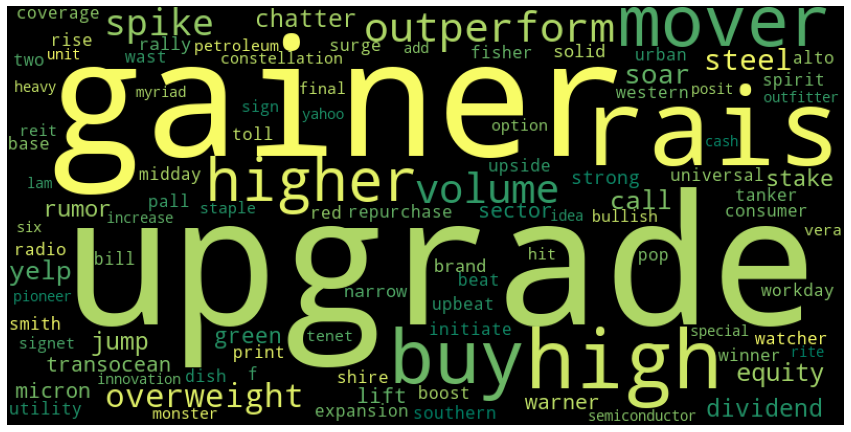
\includegraphics[scale=0.4]{pics/positive.png}
\caption{Positive words}
\end{subfigure}

\begin{subfigure}[b]{\textwidth}
\centering
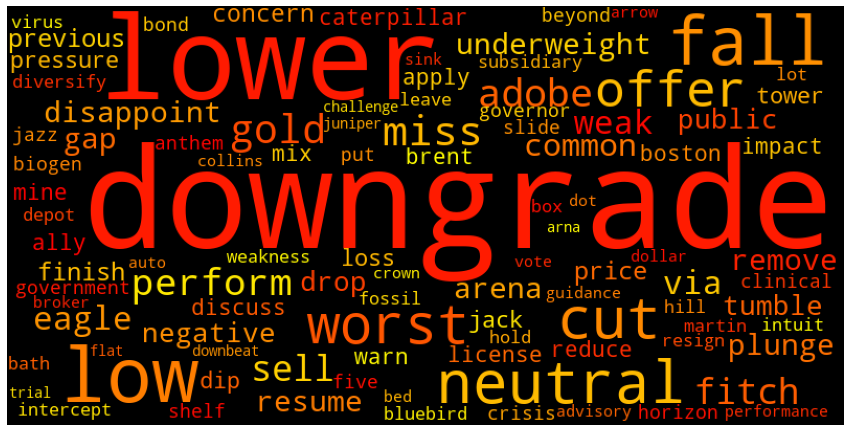
\includegraphics[scale=0.4]{pics/negative.png}
\caption{Negative words}
\end{subfigure}
\caption{Word clouds demonstrating sentiment charged words. Font size corresponds to average tone across all training samples}
\label{wordclouds}
\end{figure}

Following the construction of matrix $O$, figure \ref{wordclouds} demonstrates the list of sentiment charged words on average over all training 19 windows. At each training and validation window, the sentiment lists are generated completely from scratch, and while there is some overlap, each list can vary significantly. The font size corresponds to the average tone (calculated by $\frac{1}{2}(O_+ - O_-)$) of the words across all windows. Of the top 50 positive sentiment words, the following appeared in more than 75\% of windows, with words highlighted in \textbf{bold} appearing in all windows:
\begin{center}
      \textit{soar, raise, high, volume,} \textbf{upgrade}
\end{center}

\noindent
The following words are the equivalent with respect to top 50 negative sentiment words:
\begin{center}
      \textit{disappoint, fall, cut, plunge, low, miss, weak,} \textbf{lower, downgrade, underweight}
\end{center}

Simply by inspection, each group appears sane, in the sense that many of the words with high values in either sentiment could be assumed. However, some words are somewhat surprising and this may offer an insight into subconsious bias that exists in writing headlines as opposed to article bodies. For example, the word \textit{volume} is, under normal circumstances, a sentiment neutral word, but according to the model generated by SESTM, is a highly positive word. Examples of headlines including this word include:
\begin{itemize}
      \item \textit{Agilent spikes to high of \$60.40 on Volume}
      \item \textit{Markets gather some momentum as volume remains light, geopolitical tension improving}
      \item \textit{Tuesday's Mid-day options for Volume Leaders}
\end{itemize}

Included in the sample are headlines from `Benzinga', which is a company that offers realtime news articles, and has a significant quantity of headlines of the form \textit{Benzinga's top upgrades} and \textit{Benzinga's volume}

The headline of a news article is often packed with more impactful words to grab the attention of a reader 

% TODO: overlap with LM and Harvard

%TODO: why are some words missing? offer some explanation on why (detailed ideally, with research to back it up)

\subsection{Speed of information Assimilation}
%TODO plot graphs of day 0 to day 7 average returns to show data assimilation

\subsection{Comparison to other methods}
%TODO create table of regression on LM and H4 dictionaries to show information not captured by each

\section{What to do}

{\bf A topic-specific chapter} 
\vspace{1cm} 

\noindent
This chapter is intended to evaluate what you did.  The content is highly 
topic-specific, but for many projects will have flavours of the following:

\begin{enumerate}
\item functional  testing, including analysis and explanation of failure 
      cases,
\item behavioural testing, often including analysis of any results that 
      draw some form of conclusion wrt. the aims and objectives,
      and
\item evaluation of options and decisions within the project, and/or a
      comparison with alternatives.
\end{enumerate}

\noindent
This chapter often acts to differentiate project quality: even if the work
completed is of a high technical quality, critical yet objective evaluation 
and comparison of the outcomes is crucial.  In essence, the reader wants to
learn something, so the worst examples amount to simple statements of fact 
(e.g., ``graph X shows the result is Y''); the best examples are analytical 
and exploratory (e.g., ``graph X shows the result is Y, which means Z; this 
contradicts [1], which may be because I use a different assumption'').  As 
such, both positive {\em and} negative outcomes are valid {\em if} presented 
in a suitable manner.

% -----------------------------------------------------------------------------

\chapter{Conclusion}
\label{chap:conclusion}

\noindent
The concluding chapter of a dissertation is often underutilised because it 
is too often left too close to the deadline: it is important to allocate
enough attention to it.  Ideally, the chapter will consist of three parts:

\begin{enumerate}
\item (Re)summarise the main contributions and achievements, in essence
      summing up the content.
\item Clearly state the current project status (e.g., ``X is working, Y 
      is not'') and evaluate what has been achieved with respect to the 
      initial aims and objectives (e.g., ``I completed aim X outlined 
      previously, the evidence for this is within Chapter Y'').  There 
      is no problem including aims which were not completed, but it is 
      important to evaluate and/or justify why this is the case.
\item Outline any open problems or future plans.  Rather than treat this
      only as an exercise in what you {\em could} have done given more 
      time, try to focus on any unexplored options or interesting outcomes
      (e.g., ``my experiment for X gave counter-intuitive results, this 
      could be because Y and would form an interesting area for further 
      study'' or ``users found feature Z of my software difficult to use,
      which is obvious in hindsight but not during at design stage; to 
      resolve this, I could clearly apply the technique of Smith [7]'').
\end{enumerate}

% =============================================================================

% Finally, after the main matter, the back matter is specified.  This is
% typically populated with just the bibliography.  LaTeX deals with these
% in one of two ways, namely
%
% - inline, which roughly means the author specifies entries using the 
%   \bibitem macro and typesets them manually, or
% - using BiBTeX, which means entries are contained in a separate file
%   (which is essentially a databased) then inported; this is the 
%   approach used below, with the databased being dissertation.bib.
%
% Either way, the each entry has a key (or identifier) which can be used
% in the main matter to cite it, e.g., \cite{X}, \cite[Chapter 2}{Y}.
%
% We would recommend using BiBTeX, since it guarantees a consistent referencing style 
% and since many sites (such as dblp) provide references in BiBTeX format. 
% However, note that by default, BiBTeX will ignore capital letters in article titles 
% to ensure consistency of style. This can lead to e.g. "NP-completeness" becoming
% "np-completeness". To avoid this, make sure any capital letters you want to preserve
% are enclosed in braces in the .bib, e.g. "{NP}-completeness".

\backmatter

\bibliography{dissertation}

% -----------------------------------------------------------------------------

% The dissertation concludes with a set of (optional) appendicies; these are 
% the same as chapters in a sense, but once signaled as being appendicies via
% the associated macro, LaTeX manages them appropriatly.

\appendix

\chapter{An Example Appendix}
\label{appx:example}

Content which is not central to, but may enhance the dissertation can be 
included in one or more appendices; examples include, but are not limited
to

\begin{itemize}
\item lengthy mathematical proofs, numerical or graphical results which 
      are summarised in the main body,
\item sample or example calculations, 
      and
\item results of user studies or questionnaires.
\end{itemize}

\noindent
Note that in line with most research conferences, the marking panel is not
obliged to read such appendices. The point of including them is to serve as
an additional reference if and only if the marker needs it in order to check
something in the main text. For example, the marker might check a program listing 
in an appendix if they think the description in the main dissertation is ambiguous.

% =============================================================================

\end{document}
